\documentclass{datamining}
\newcommand\datasize{280}
\newcommand\trainingsetsize{230}
\newcommand\validationsetsize{50}
\newcommand\testingsetsize{80}
\newcommand\timestamp{3. 4. 2025 13:07:21}
\newcommand\trainingtime{00:00:05}

\usepackage{xcolor}                % Custom colors
\usepackage{tikz}                  % For full-width color boxes
\usetikzlibrary{calc}
\usepackage{lipsum}                % Dummy text
\usepackage{tabularx}
\usepackage{graphicx}

\graphicspath{ {images/} }

% Define custom colors
\definecolor{darkblue}{HTML}{003366}
\definecolor{lightblue}{HTML}{6699CC}

\renewcommand{\arraystretch}{1.5} 

\begin{document}
	\begin{center}
		\LARGE{Report k případové studii} \\
		\large{Doporučení léčebné metody}
	\end{center}
	
	\section{Souhrn}
	\begin{tabularx}{\textwidth}{|>{\hsize=.75\hsize}X|>{\hsize=.25\hsize}X|}	
		\hline
		Časové razítko & \timestamp \\
		\hline
		Doba trénování & \trainingtime \\
		\hline
	\end{tabularx}
	\section{Informace o datech}
	
	\begin{tabularx}{\textwidth}{|>{\hsize=.5\hsize}X|>{\hsize=.5\hsize}X|}	
		\hline
		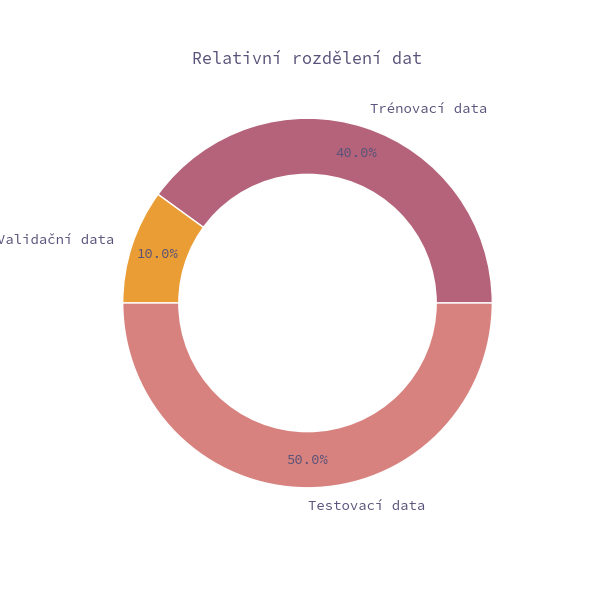
\includegraphics[width=0.9\hsize]{training_data_split}
		 &
		 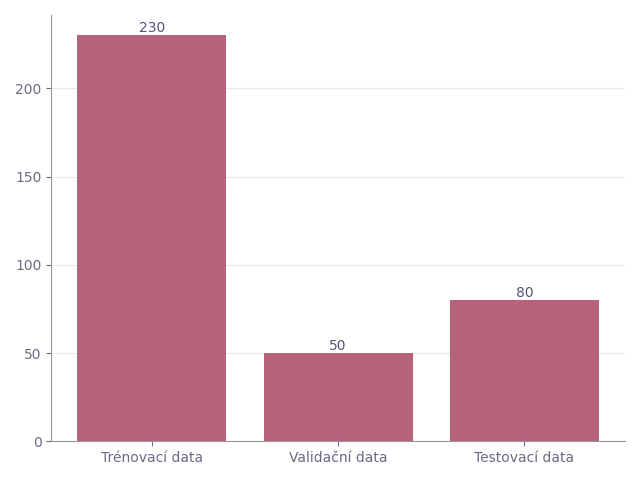
\includegraphics[width=0.9\hsize]{training_data_histogram}
		 \\
		\hline
		Relativní rozdělení dat & Absolutní rozdělení dat \\
		\hline
	\end{tabularx}
	\vspace{2cm}
\end{document}